\chapter{Bitácora}
\label{bitacora}


\subsection{Estructura de almacenamiento de
datos}\label{estructura-de-almacenamiento-de-datos}

Los archivos originales vienen agrupados por libro y por tipo de datos.
Hay una carpeta por cada libro y dentro de ella hay una carpeta con los
PDFs (\texttt{libro/pdf}) y otra con los JPGs (\texttt{libro/jpg}). Por
lo tanto, decidimos almacenar los textos en una carpeta por separado
(\texttt{libro/txt}), con los nombres correspondientes de los PDFs pero
con terminación \texttt{.txt}. Adicionalmente, dentro de la carpeta de
los textos hay una carpeta con el contenido completo del libro en un
solo archivo (\texttt{libro/txt/full/libro.txt}). Más adelante
describiremos cómo es que extrajimos los textos de los PDFs, pero por lo
pronto, la estructura de las carpetas quedó como sigue:

\textbf{Carpeta global con todo el contenido}

\begin{itemize}
\itemsep1pt\parskip0pt\parsep0pt
\item
  Carpeta de un libro
\item
  \emph{PDF} Un archivo \texttt{.pdf} por página
\item
  \emph{JPG} Un archivo \texttt{.jpg} por página
\item
  \emph{TXT} Un archivo \texttt{.txt} por página con el mismo nombre que
  los PDFs
\item
  \emph{Full} Un solo archivo \texttt{.txt} con el mismo nombre del
  libro
\end{itemize}

\subsection{ELT}\label{elt}

En esta sección describiremos el proceso que seguimos para la
extracción, carga y transformación de los datos. Procesar correctamente
los datos es parte crucial del proyecto, pues los algoritmos tienen como
insumo la información procesada.

\subsubsection{{[}E{]} Extracción de textos a partir de los
PDFs}\label{e-extraccion-de-textos-a-partir-de-los-pdfs}

Hicimos varios códigos en \texttt{bash} alrededor del comando
\texttt{pdftotext} para extraer los textos contenidos como metadatos en
los PDFs. Originalmente generamos códigos locales para pruebas que
extraen los textos de una colección de datos en el formato descrito
arriba y ponen los textos en su lugar correspondiente.

Tenemos dos versiones:

\begin{itemize}
\item
  Versión básica (\texttt{parallel\_pdftotext.sh}): Toma una carpeta con
  PDFs y los extrae en una carpeta objetivo. Además, lo hace en paralelo
  para aprovechar los diversos núcleos de la máquina. Este script es
  multipropósito y podrá ser utilizado por ejemplo al agregar nuevos
  libros a la colección.
\item
  Versión masiva (\texttt{mass\_pdftotext.sh}): Recibe la carpeta con
  todos los libros y utiliza la versión básica para extraer los textos
  en la carpeta correspondiente de cada libro.
\end{itemize}

Adicionalmente, el script \texttt{full\_txt.sh} recibe el árbol completo
de carpetas, pega los textos de cada libro y pone el resultado en la
carpeta \texttt{libro/txt/full}.

Dado que los PDFs de la colección ocupan aproximadamente 400 GB, puede
resultar complicado y/o caro manejarlos todos. Para ello también creamos
dos scripts que suponen que la información está en S3 y van bajando y
borrando la información libro a libro con el fin de ahorrar espacio en
la máquina local en la que se está procesando la información:

\begin{itemize}
\item
  El primer script (\texttt{s3\_pdftotext.sh}) baja los PDFs libro a
  libro y los extrae en una carpeta local, preservando la estructura
  deseada de los archivos. Es similar al script local masivo, pero la
  diferencia es que la información original está en S3. Después de
  procesar cada libro (las páginas se procesan en paralelo), borra los
  PDFs que se bajaron y de este modo sólo se necesita un disco con
  capacidad = tamaño del libro más grande + tamaño total de los textos.
  Después de este paso se debe correr también \texttt{full-txt.sh} si se
  quiere tener la versión completa (en lugar de por página) de los
  libros.
\item
  El segundo script (\texttt{s3\_upload\_txt.sh}) sube los resultados
  obtenidos en el script de conversión a texto a una carpeta en S3. La
  ventaja es que preserva la estructura de los archivos, por lo que
  basta correr el script de bajada una vez y el de subida una vez y ya
  está la colección de textos agregada en S3.
\end{itemize}

\subsubsection{{[}LT{]} Conversión a formato apropiado para minería de
textos}\label{lt-conversion-a-formato-apropiado-para-mineria-de-textos}

La limpieza se puede llevar a cabo en \texttt{bash}. Sin embargo, hay
algunas operaciones más sofisticadas que queremos hacer que sólo están
en R. Por eso optamos por hacer la limpieza en R siguiendo los
siguientes pasos:

\begin{enumerate}
\def\labelenumi{\arabic{enumi}.}
\itemsep1pt\parskip0pt\parsep0pt
\item
  {[}L{]} Cargamos los datos a un \texttt{Corpus} del paquete
  \texttt{tm} (Text Mining).

  \begin{itemize}
  \itemsep1pt\parskip0pt\parsep0pt
  \item
    Cada libro corresponde a un documento.
  \end{itemize}
\end{enumerate}

\begin{itemize}
\itemsep1pt\parskip0pt\parsep0pt
\item
  Hay una lista negra de libros cuyos \texttt{.txt} están demasiado mal.
  Dejarlos llena el diccionario de términos conocidos de basura.

  \begin{itemize}
  \itemsep1pt\parskip0pt\parsep0pt
  \item
    Detectamos el idioma del libro con el paquete \texttt{textcat}.
  \item
    Sólo permitimos español, inglés, francés, alemán, portugués e
    italiano.
  \item
    Hay pocos libros en latín y catalán que ignoramos al menos por
    ahora. Hacerlo disminuye mucho el problema computacional.
  \item
    Llenamos las partes relevantes de los metadatos, que en este caso
    son el nombre del libro y el idioma.
  \end{itemize}
\end{itemize}

\begin{enumerate}
\def\labelenumi{\arabic{enumi}.}
\setcounter{enumi}{1}
\itemsep1pt\parskip0pt\parsep0pt
\item
  {[}T{]} Transformamos los datos a un formato apropiado para la
  minería:

  \begin{itemize}
  \itemsep1pt\parskip0pt\parsep0pt
  \item
    Limpiamos los datos:

    \begin{itemize}
    \itemsep1pt\parskip0pt\parsep0pt
    \item
      Quitamos caracteres especiales, puntuación, exceso de espacios,
      etc.
    \item
      Hacemos \emph{stemming}: tomamos únicamente las raíces de las
      palabras pero ignoramos las terminaciones. Los experimentos
      sugieren que tal vez convenga \emph{no} hacer stemming, aunque
      esto representa un reto técnico (ver sección de Estadísticas
      abajo).
    \end{itemize}
  \item
    Generamos un Corpus limpio con metadatos.
  \item
    Finalmente, generamos la matriz de términos-documentos
  \item
    Quitamos las palabras que no aparezcan al menos en 2 documentos.

    \begin{itemize}
    \itemsep1pt\parskip0pt\parsep0pt
    \item
      Así evitamos que las palabras mal leídas se queden en el
      diccionario.
    \end{itemize}
  \item
    En este punto podemos quitar ``stopwords'', es decir palabras
    inconsecuentes como ``el'', ``la'', etc.
  \item
    Los pesos están dados según la aplicación:

    \begin{itemize}
    \itemsep1pt\parskip0pt\parsep0pt
    \item
      Para tópicos usamos frecuencias (TF) y hacemos el análisis
      \emph{por libro}.
    \item
      Para búsquedas usamos TF-IDF y hacemos el análisis \emph{por
      página}.
    \end{itemize}
  \end{itemize}
\end{enumerate}

Cabe mencionar que como R hace todo en memoria, hacer el proceso
anterior para la colección entera de textos es demasiado pesado. Sin
embargo, dado que se puede procesar los textos independientemente unos
de otros, optamos por procesarlos en \emph{batches} de un tamaño fijo
(digamos 20,000 textos en el caso de que sea por página) y guardar tanto
los \texttt{Corpus} limpios como sus matrices términos-documentos
asociadas en archivos \texttt{.Rdata}. La ventaja de esto es que
\texttt{tm} tiene manera de concatenar los \texttt{Corpus} y las
matrices, de modo que se puede procesar por partes y luego juntar la
información procesada sin problemas.

Dado que la matriz de términos documentos es toda la información que
necesitan los algoritmos para correr, bastará subir la matriz a la
memoria para hacer recomendaciones.

\subsubsection{Ejemplo de limpieza}\label{ejemplo-de-limpieza}

El texto original se ve así (extracto):

\begin{lstlisting}
##   Actualmente es becario de Jovenes Creadores del Fondo Nacional para la Cultura y las Artes.
##        Su obra forma parte de importantes coleccciones como la del Instituto de Artes Graficas de Oaxaca; Museo Universitario
##   Contemporaneo de Arte, Museo Panstowe, Majdanek, Polonia; Casa de las Americas de la Habana, Cuba; Museo Jose Guadalupe
##   Posada de la ciudad de Aguascalientes.
\end{lstlisting}

Después de haberle quitado la puntuación y las mayúsculas:

\begin{lstlisting}
 ## actualmente es becario de jovenes creadores del fondo nacional para la cultura las artes su obra forma parte de importantes coleccciones como la del instituto de artes graficas de oaxaca museo universitario contemporaneo de arte museo panstowe majdanek polonia casa de las americas de la habana cuba museo jose guadalupe posada de la ciudad de aguascalientes
\end{lstlisting}

Después de hacer \emph{stemming}:

\begin{lstlisting}
 ## bec de la fundacion mexam par resident artist en vermont studi cent estad unid actual es becari de joven creador del fond nacional par la cultur las artes su obra form part de import colecccion com la del institut de artes grafic de oaxac muse universitari contemporane de arte muse panstow majdanek poloni cas de las amer de la haban cub muse jos guadalup pos de la ciud de aguascalient
\end{lstlisting}

Y si quitamos las \emph{stopwords}:

\begin{lstlisting}
 ## bec fundacion mexam par resident artist vermont studi cent unid actual becari joven creador fond nacional par cultur artes obra form part import colecccion com institut artes grafic oaxac muse universitari contemporane arte muse panstow majdanek poloni cas amer haban cub muse jos guadalup pos ciud aguascalient
\end{lstlisting}

\subsubsection{Estadísticas básicas}\label{estadisticas-basicas}

A continuación presentamos algunos datos básicos sobre la colección
después de haberla limpiado y de haber quitado los textos de mala
calidad.

\begin{itemize}
\itemsep1pt\parskip0pt\parsep0pt
\item
  Número de documentos: 1335
\item
  Número de términos: 414342
\item
  Tamaño del Corpus después del stemming (archivo .Rdata):
  \textasciitilde{} 170 MB
\item
  Tamaño de la matriz términos-documentos (archivo .Rdata):
  \textasciitilde{} 40 MB
\item
  Longitud del término más largo: 25
\item
  Mínimo número de documentos en los que tiene que aparecer un término
  para ser tomado en cuenta: 2
\end{itemize}

A continuación presentamos un histograma del número de palabras por
libro:

\begin{figure}[H]
\centering
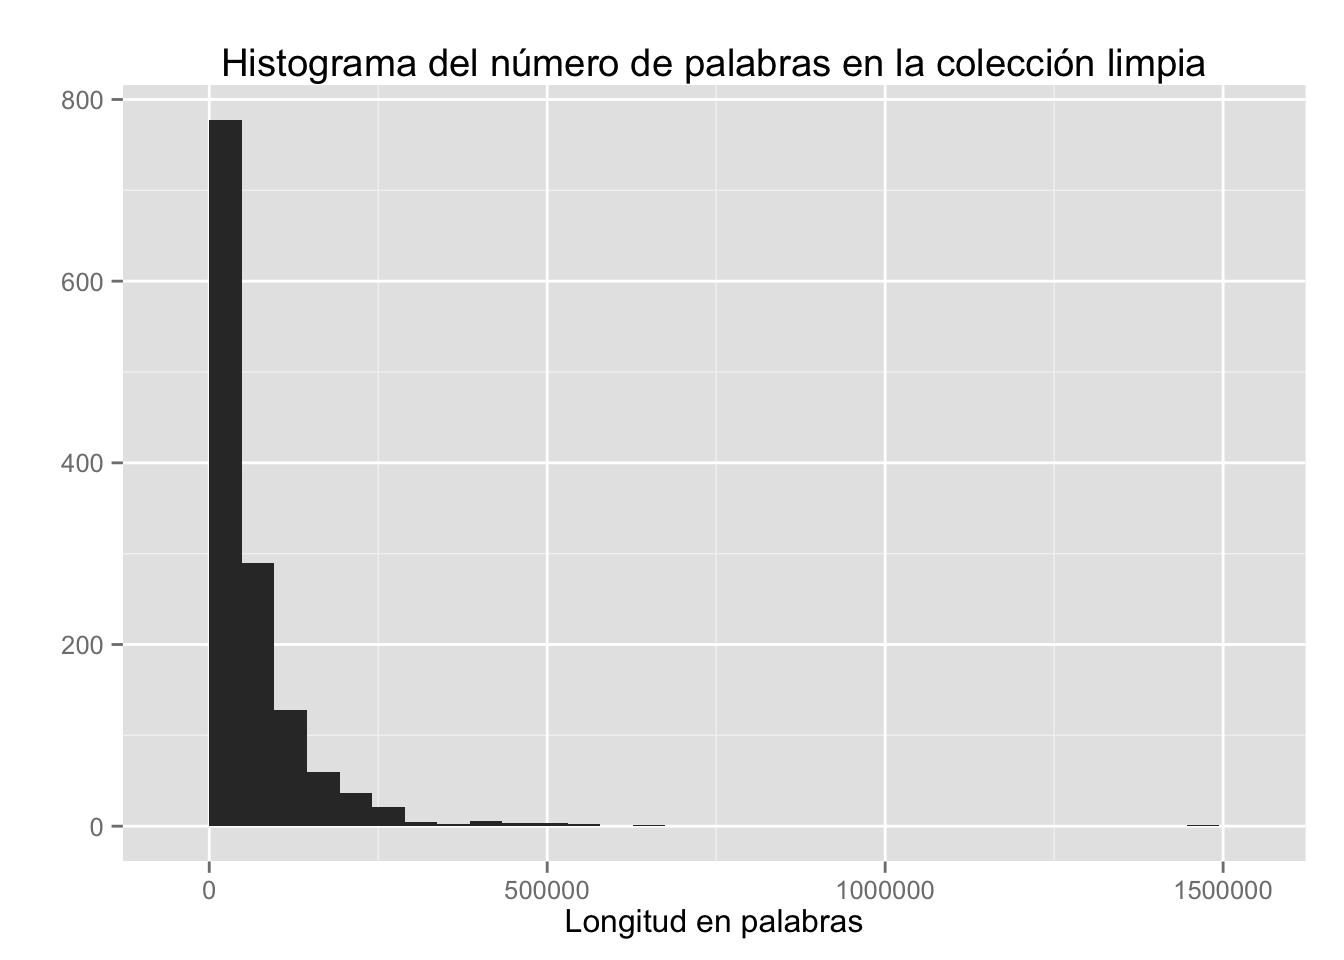
\includegraphics[width=1\textwidth]{Figures/L1.png}
\caption{Histograma palabras por libro}
\end{figure}

Y ahora una tabla con el número de documentos en cada idioma. Cabe notar
que aquí ya sólo están los documentos en los idiomas permitidos y que no
están en la lista negra.

\begin{figure}[H]
\centering
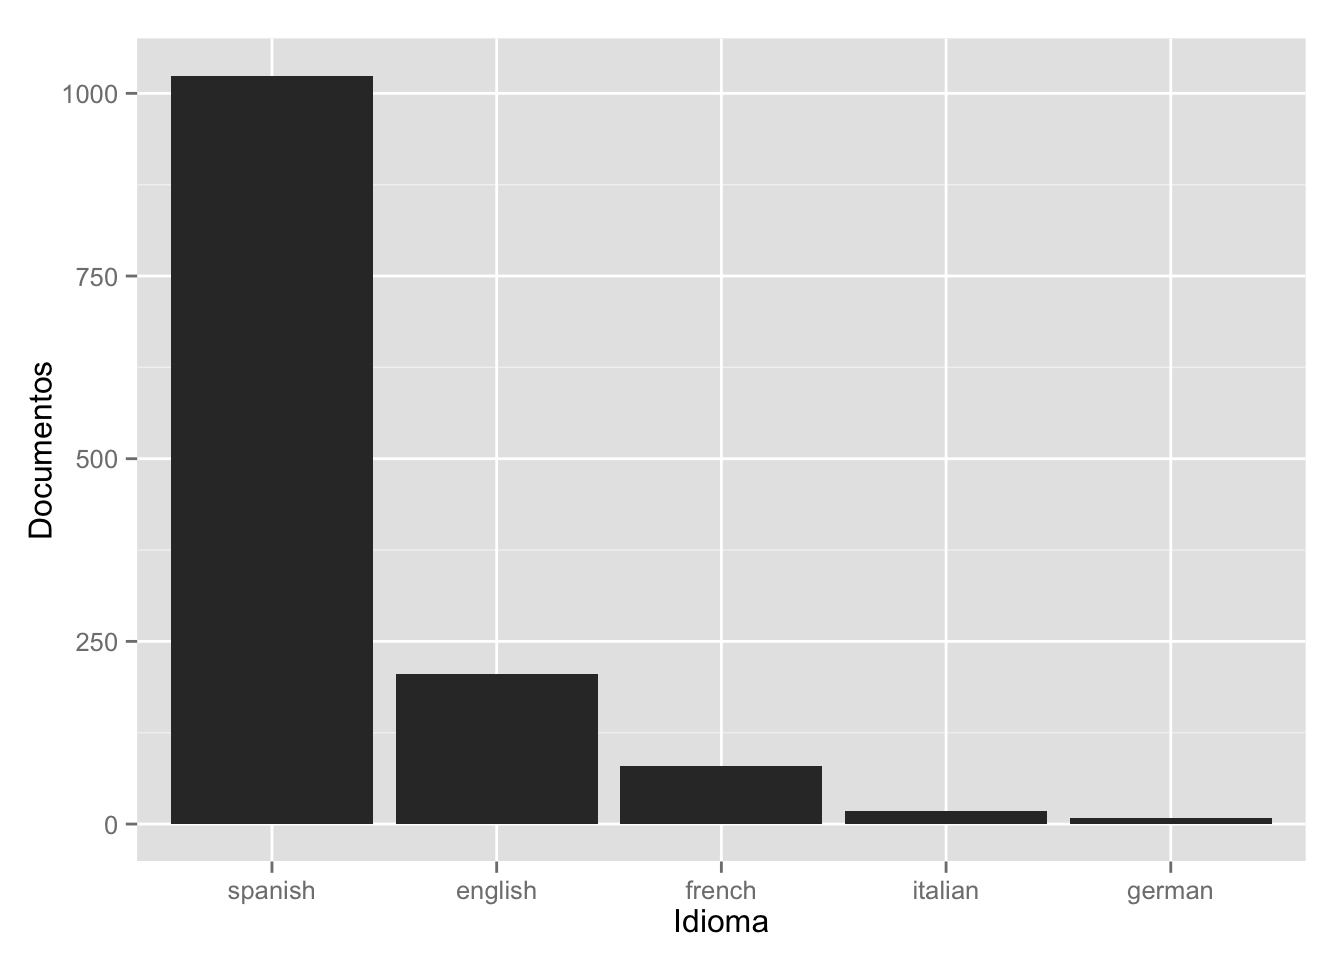
\includegraphics[width=1\textwidth]{Figures/L2.png}
\caption{}
\label{}
\end{figure}

\begin{table}[]
\centering
\begin{tabular}{@{}ll@{}}
\toprule
\textbf{Idioma} & \textbf{Documentos} \\ \midrule
spanish         & 1024                \\
english         & 206                 \\
french          & 79                  \\
italian         & 18                  \\
german          & 8                   \\ \bottomrule
\end{tabular}
\caption{Análisis de documentos}
\label{my-label}
\end{table}


\subsubsection{Análisis de palabras}\label{analisis-de-palabras}

A continuación se muestra un breve análisis de las palabras más y menos
frecuentes. Como aplicamos \emph{stemming} en realidad lo que estamos
analizando es cuáles son las raíces más comunes. Las más frecuentes son:

\begin{table}[]
\centering
\caption{Análisis de palabras}
\label{my-label}
\begin{tabular}{ll}
\textbf{Palabras} & \textbf{Frecuencia} \\
tod               & 287987              \\
sobr              & 146383              \\
part              & 139525              \\
hac               & 134778              \\
mism              & 127777              \\
sol               & 123630              \\
ser               & 123435              \\
mexic             & 110228              \\
algun             & 110104              \\
bien              & 103034              \\
form              & 102238              \\
san               & 100928              \\
cas               & 100205              \\
much              & 95109               \\
pued              & 93597               \\ \hline
\end{tabular}
\end{table}


\begin{figure}[H]
\centering
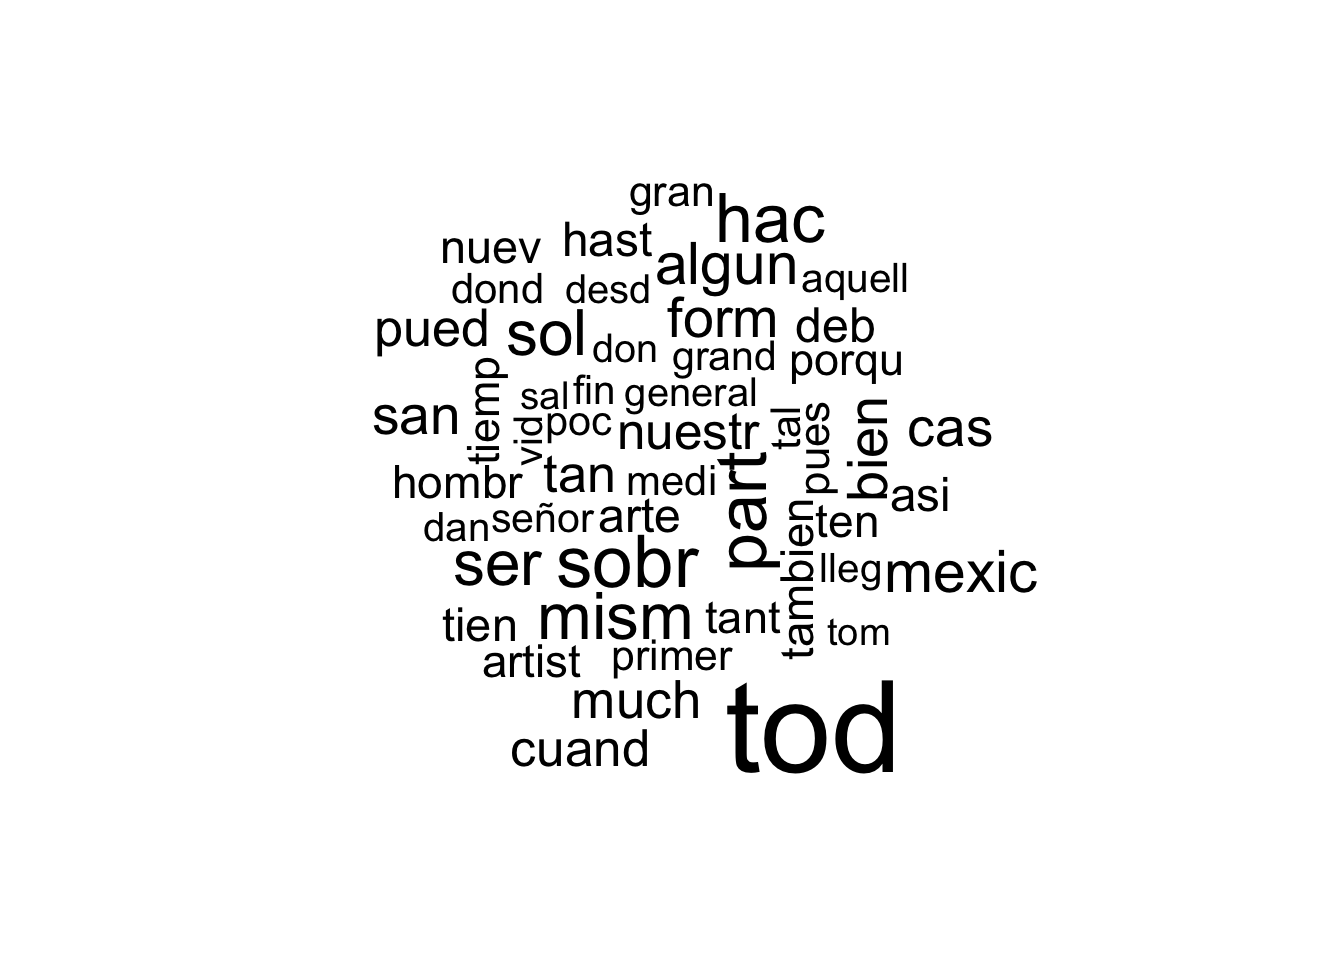
\includegraphics[width=1\textwidth]{Figures/L6.png}
\caption{imagen5}
\end{figure}



La gran mayoría de las palabras aparecen menos de 50 veces:

\begin{figure}[H]
\centering
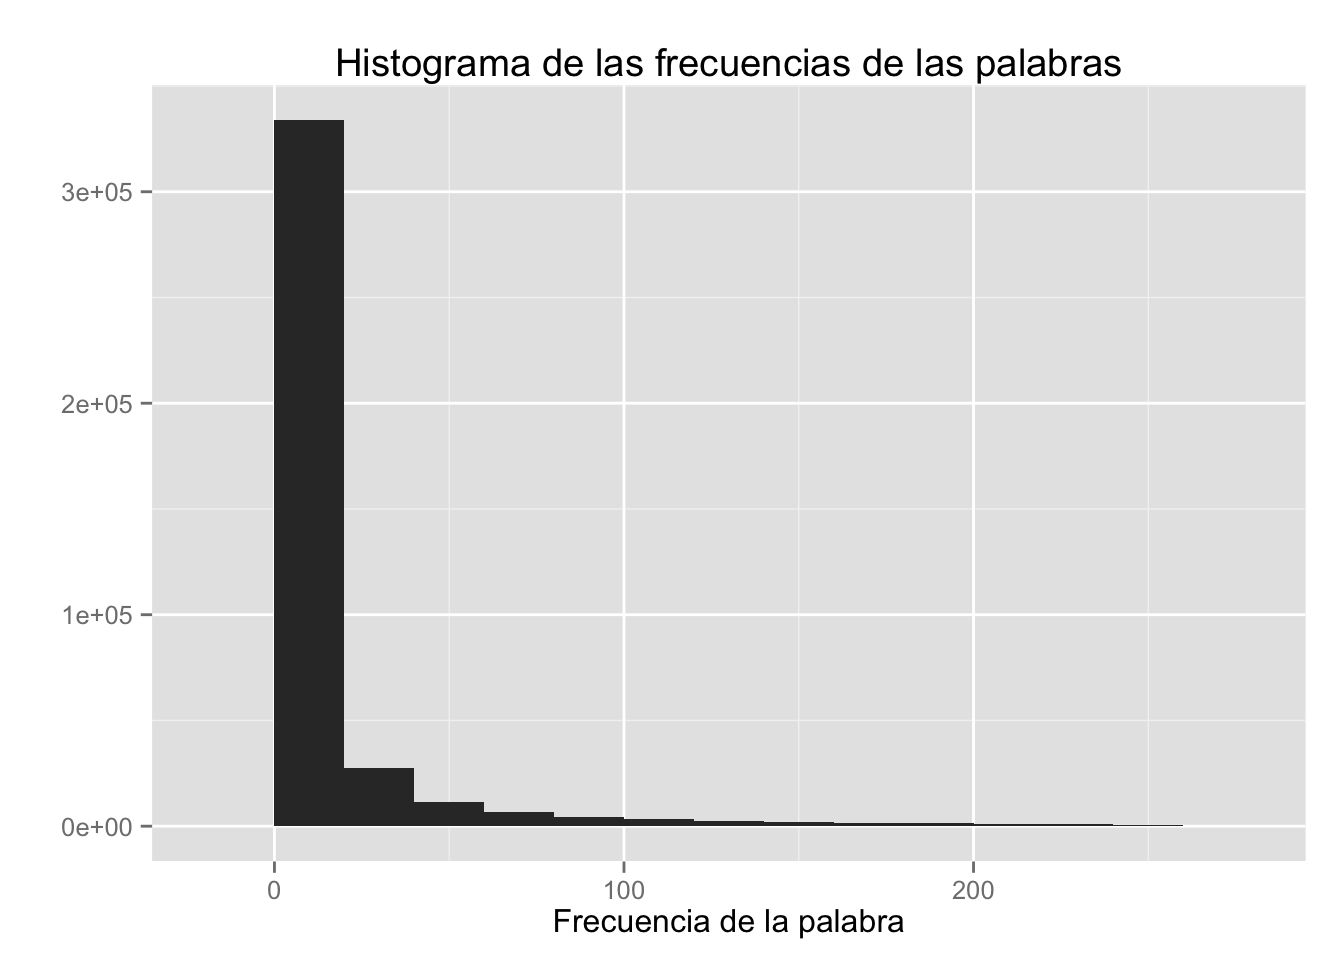
\includegraphics[width=1\textwidth]{Figures/L3.png}
\caption{imagen5}
\label{}
\end{figure}

\subsubsection{Notas}\label{notas}

Hemos tenido algo de problemas con la decisión de si debemos hacer
stemming o no. La ventaja del stemming es que permite que las búsquedas
sean más difusas, es decir, que tome como iguales a las palabras con las
mismas raíces. Sin embargo, esto viene con dos problemas. El primero es
que hay palabras con significados distintos pero raíces iguales, y el
segundo es que al quitar las raíces, a veces se pierden partes
distintivas del lenguaje de la búsqueda. Ambos problemas generan falsos
positivos. El tema es que si no se hace stemming, hay otras
complicaciones. Por ejemplo, la búsqueda es tan exacta que puede parecer
tonta (por ejemplo no considera como iguales a una palabra y su plural).
Otro problema es que dado que se manejan varios lenguajes y todos
contribuyen al diccionario de palabras conocidas, éste puede hacerse
enorme (alrededor de \#FALTA\# 5 millones de palabras) y resultar
demasiado pesado para un sistema que corra en vivo.

%%%%%%%%%%%%%%%%%%%%%%%%%%%%%%%%%%%%%%%%%%%%%%%%%%%%%%
%%%%%%%%%%%%%%%%%%%%%%%%%%%%%%%%%%%%%% FELIPE  por favor meter parrafito de LSI

\subsubsection{Tópicos automáticos: LDA} \label{topicos-automaticos-lda}

Se utilizó la técnica conocida cómo \emph{LDA} para
extraer los tópicos o temas relevantes de los textos. Creemos que es
mejor hacer la extracción de los tópicos a nivel de libro ya que los
libros se tratan de un tema en particular. También estamos investigando
si es posible extraer subtópicos, es decir una especie de tópicos
jerarquizados o bien si es posible mapear más de un tema a cada
documento.

Se han realizado pruebas para ver la efectividad de esta técnica,
cambiando el parámetro del número de tópicos, sin embargo este depende
de cada texto, por lo que estamos tratando de inferir un parámetro
adecuado. También se propone dentro del análisis utilizar el corpus sin
\emph{stemming} ya que no se interpreta con facilidad el tema y
consideramos que es mejor así.



\subsubsection{Búsqueda inteligente:
TF-IDF}\label{busqueda-inteligente-tf-idf}


La técnica TF-IDF es un
método para calcular similitudes entre textos. Dado un texto, busca los
textos más parecidos en una colección de otros textos. Para hacerlo se
basa en dos premisas básicas:

\begin{enumerate}
\def\labelenumi{\arabic{enumi})}
\itemsep1pt\parskip0pt\parsep0pt
\item
  Si dos textos tienen muchas ocurrencias de la misma palabra, significa
  que se se parecen.
\item
  Si una palabra es poco común, entonces que dos textos la contengan
  aumenta su similitud más que si contienen palabras comunes.
\end{enumerate}

La idea es entonces utilizar la consulta como ``texto'' y ver cuáles de
los de la colección son los más parecidos. El resultado es que si
buscamos con algunas palabras, el algoritmo nos traerá las páginas más
relevantes a esos términos.


Para la extracción del texto se ejecutó un algoritmo que extrae en paralelo el texto de cada documento PDF. Este proceso depende de las distintas tipografías que se encuentran en cada documento. Esto implica que en este proceso aparecen caracteres \textbf{raros} y con todo tipo de codificaciones. Por lo anterior, se decidió que la unidad de análisis es una página. 


El pipeline completo del minado de textos quedaría entonces como sigue:

\begin{enumerate}
\def\labelenumi{\arabic{enumi}.}
\itemsep1pt\parskip0pt\parsep0pt
\item
  \textbf{Procesamiento inicial}:

  \begin{enumerate}
  \def\labelenumii{\alph{enumii}.}
  \itemsep1pt\parskip0pt\parsep0pt
  \item
    Dependiendo de dónde se almacenen los archivos, correr los scripts
    en \texttt{bash} correspondientes para extraer los textos. En el
    caso de que estén en la nube de Amazon, se puede decidir subirlos de
    vuelta.
  \item
    Limpiar el \texttt{Corpus} inicial por \emph{batches} para evitar
    saturar la máquina utilizando el script de R.
  \item
    Generar las matrices términos-documentos necesarias para los
    algoritmos (en R).
  \item
    Generar los tópicos con LDA (en R).
  \end{enumerate}
\item
  Se puede utilizar conjuntamente los tópicos y las matrices resultantes
  del paso (1) para \textbf{buscar}. El servidor necesita tener R para
  poder hacer búsquedas.
\item
  Para \textbf{agregar libros nuevos} a la colección se debe llevar a
  cabo los siguientes pasos:

  \begin{enumerate}
  \def\labelenumii{\alph{enumii}.}
  \itemsep1pt\parskip0pt\parsep0pt
  \item
    Extraer los textos con el script más conveniente. Si es un libro
    puede ser con el básico; si es una colección local puede hacerse con
    el masivo, etc.
  \item
    Limpiar el \texttt{Corpus} y las matrices de términos-documentos del
    nuevo conjunto de datos.
  \item
    Combinar el \texttt{Corpus} y las matrices nuevas con los
    preexistentes para obtener la colección actualizada.
  \end{enumerate}
\end{enumerate}




Las colecciones grandes de documentos pueden ser difíciles de aprovechar. Por ejemplo, si queremos que una o varias palabras aparezcan en el documento, podemos hacer un filtro simple. Sin embargo, si las palabras son (razonablemente) comunes, el query nos podría regresar un porcentaje importante de la colección de documentos, sobre todo si son muy largos. Algo más refinado que podríamos hacer sería por ejemplo usar el número de veces que aparecen las palabras deseadas, aunque esto favorecería documentos extensos y las palabras comunes.

El conjunto de datos es interesante porqué provee las versiones cortas de los artículos, de modo que podemos leerlos y darnos una idea rápida de lo que trata cada artículo. Con la información en crudo (.txt) podemos utilizar la información cruda  para hacer el proceso desde la limpieza de los datos. El objetivo es realizar búsquedas temáticas inteligentes dentro de la colección, es decir, dado un conjunto de palabras clave, queremos obtener los artículos más relevantes. En la siguiente sección describiremos la teoría del método que utilizamos para mitigar los problemas descritos anteriormente.


